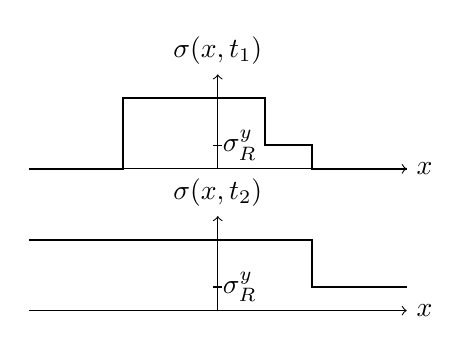
\begin{tikzpicture}[scale=0.6]
\draw[->] (0,0) -- (0,2) node [above] {$\sigma(x,t_1)$};
\draw[->] (-4,0) -- (4,0) node [right] {$x$};
\draw[thick] (-4,0) --(-2,0) -- (-2,1.5) -- (-0,1.5) -- (-0,1.5) -- (1,1.5) -- (1,0.5) -- (2,0.5) -- (2,0) -- (4,.0);
\draw (-0.1,0.5) node[right] {$\sigma_R^y$}-- (0.1,0.5);

\draw[->] (0,0-3) -- (0,2-3) node [above] {$\sigma(x,t_2)$};
\draw[->] (-4,0-3) -- (4,0-3) node [right] {$x$};
\draw[thick] (-4,1.5-3)  -- (-0,1.5-3)  --(-0,1.5-3) -- (2,1.5-3) -- (2,.5-3) -- (4,.5-3);
\draw (-0.1,0.5-3) node[right] {$\sigma_R^y$}-- (0.1,0.5-3);

\end{tikzpicture}